\section{Injection and removal of CH$_3$T}

Two CH$_3$T sources with total activities of 3 Bq and 200 Bq were prepared for use in LUX. Each source is contained in a 2.25 liter stainless steel bottle and is mixed with 2 atmospheres of LUX-quality purified xenon. The xenon acts as a carrier gas to extract the source from the bottle. The CH$_3$T was synthesized by Moravek Biochemical~\cite{moravek} and delivered at a specific activity of 0.1 milliCurie per millimol.

The injection system is shown in Fig.~\ref{fig:plumbing}. A fraction of the source bottle activity may be extracted by allowing the carrier gas to expand into one or more expansion volumes consisting of various sections of evacuated tubing. The amount of extracted activity is controlled by selecting an expansion volume of appropriate size. A methane purifier (SAES model MC1-905F\cite{seas}) located between the source bottle and the expansion volume ensures that only CH$_3$T, CH$_4$, and noble gases are allowed to enter the system. The extracted activity is then injected into the TPC by diverting a small portion of the LUX xenon gas flow through the expansion volumes. 

\begin{figure}[t!]
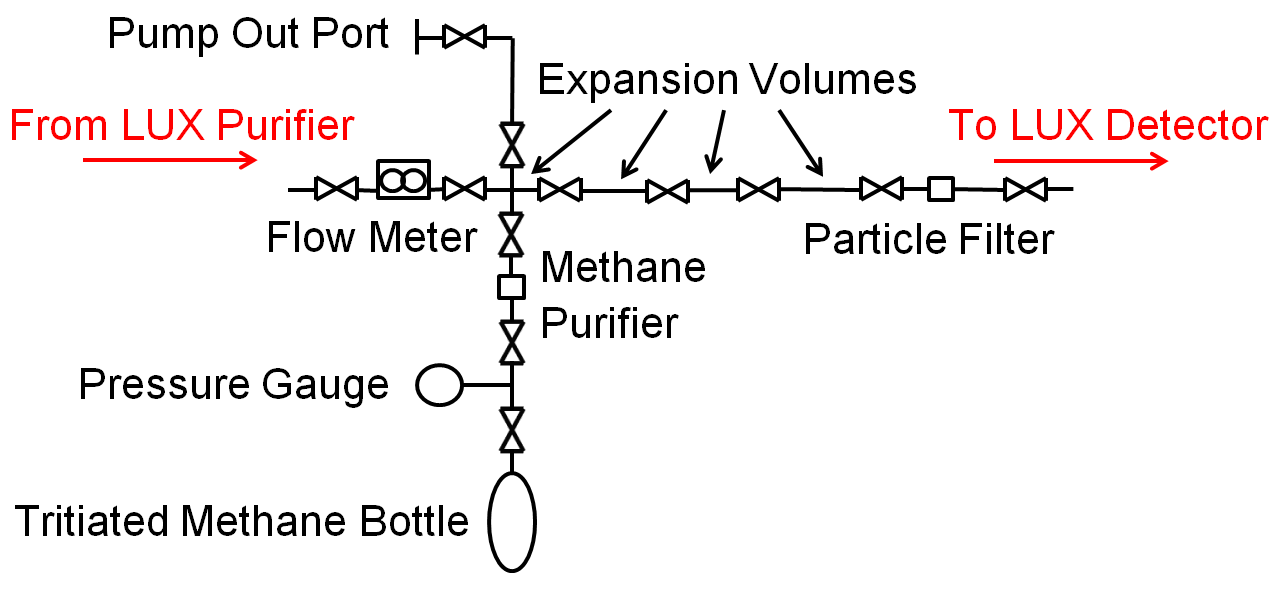
\includegraphics[width=80mm]{fig/fig1.png}
\caption{Plumbing diagram of the CH$_3$T injection system for LUX. CH$_3$T is injected downstream of the xenon gas purifier so that it passes through the detector prior to being removed.  Red arrows indicate the direction of flow.}
\label{fig:plumbing}
\end{figure}

The CH$_3$T appears in the TPC within minutes of the injection, and is removed via the normal action of the LUX xenon purification system, which operates without interruption during the entire procedure. Its centerpiece is a hot zirconium getter (SAES model PS4-MT15-R1\cite{seas}) that acts upon gaseous xenon and continuously removes all non-noble species including methane. The xenon gas flow is driven by a diaphragm pump at a rate of $\sim$27 standard liters per minute (slpm). 


\begin{figure}[t!]
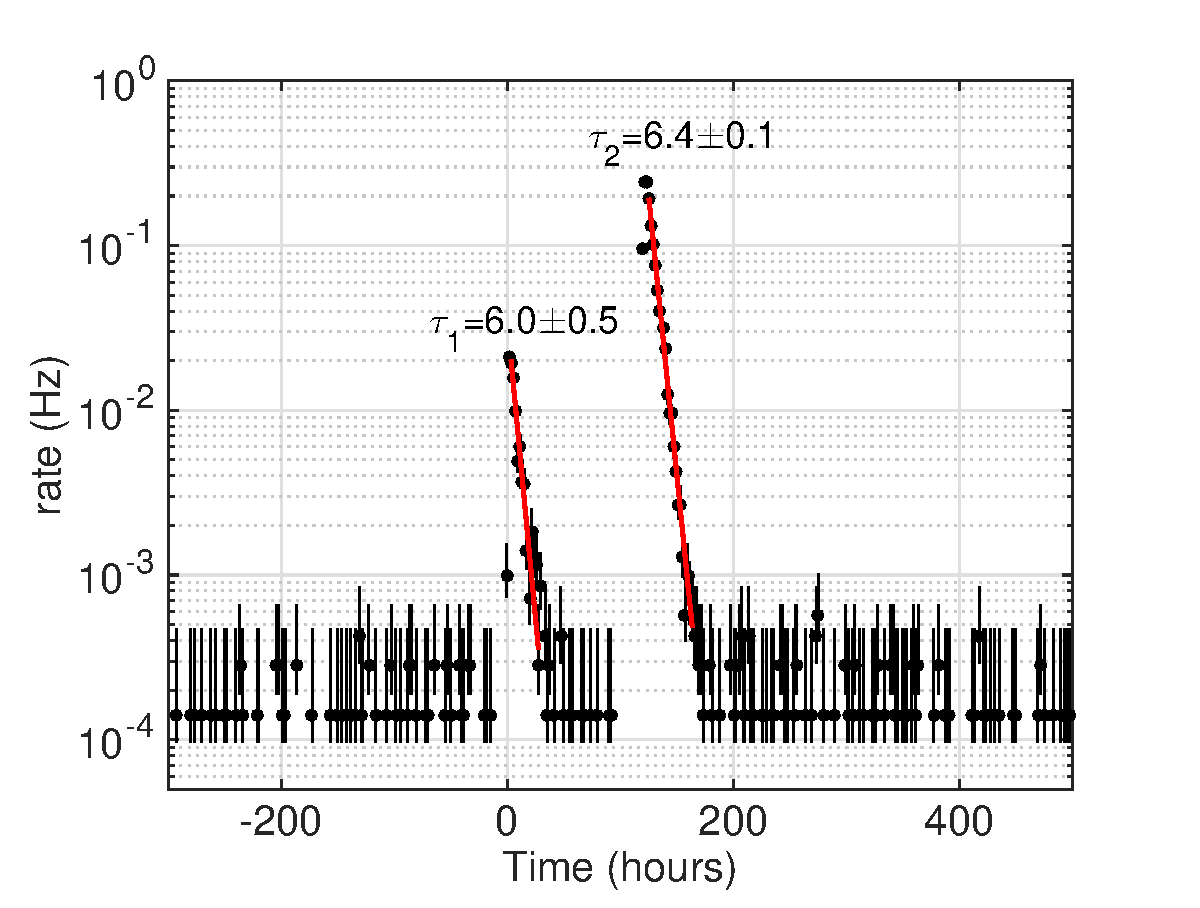
\includegraphics[width=90mm]{fig/fig2.eps}
\caption{Rate of single scatter events with S1 below 150 phd in the fiducial volume during the August 2013 CH$_3$T injections.  The solid lines are exponential fits to the activity vs. time.}
\label{fig:ch3t_removal}
\end{figure}


 
\begin{figure}[t!]
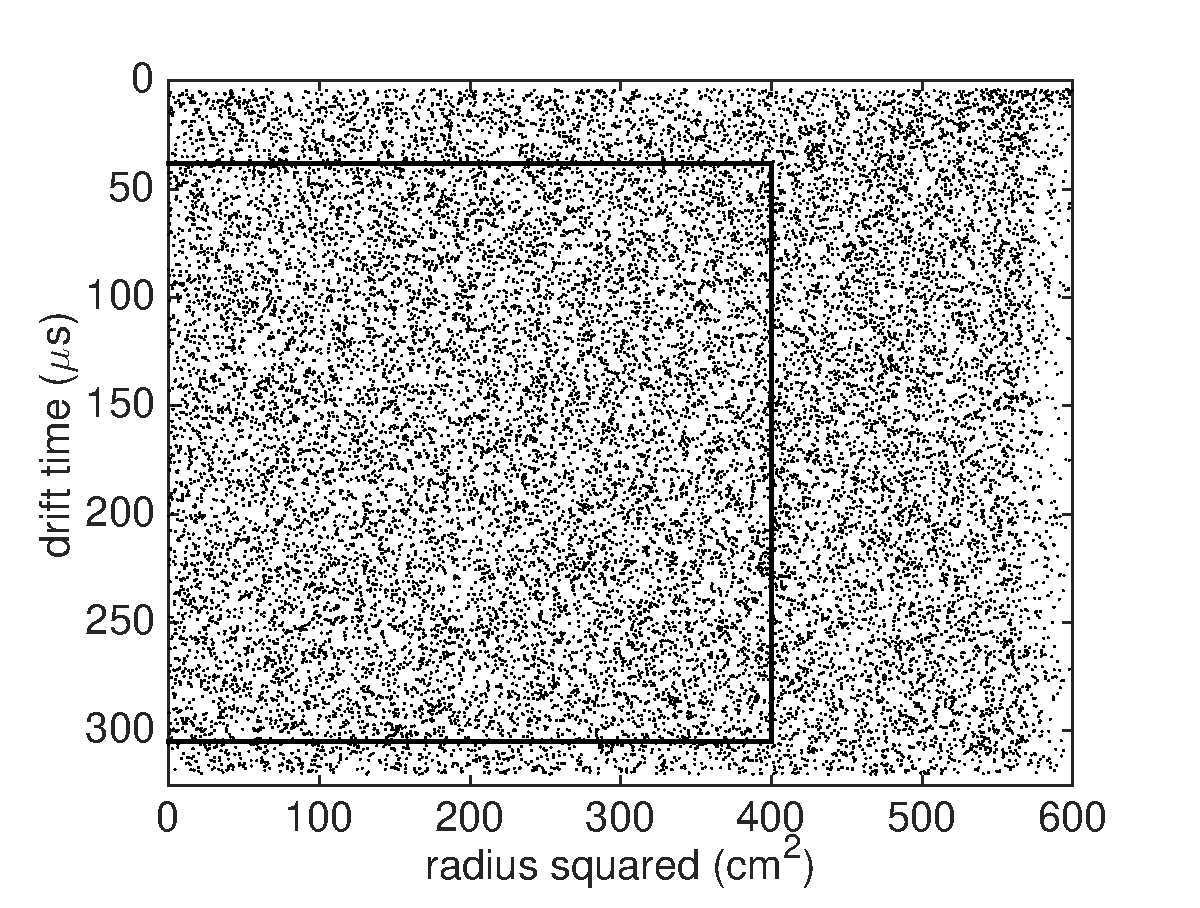
\includegraphics[width=90mm]{fig/fig3.eps}
\caption{The location of events in drift time vs. detector radius squared for the August 2013 CH$_3$T injection. The drift time is a proxy for the $z$ coordinate of the event. The solid black line represents the fiducial volume used in Ref.~\cite{lux-reanalysis}.}
\label{fig:event_location}
\end{figure}


Prior to the first injection of CH$_3$T activity, we first confirmed that the LUX getter unit was capable of efficient methane removal by injecting  $\sim$1 ppm (part-per-million g/g) of natural methane (CH$_4$) into LUX. As shown in Appendix~\ref{sec:appendix1}, the CH$_4$ concentration in the gas, monitored with a mass spectrometer, was observed  to decrease exponentially with a time constant of 5.9 $\pm 0.07$ hours. The one-pass efficiency of the getter for CH$_4$ removal was measured to be 97\% under the LUX flow and temperature conditions by sampling the gas before and after the getter. 

On August 8, 2013, an initial injection of 20 mBq of CH$_3$T was performed, followed five days later by an injection of 800 mBq. The count rate of fiducial single-scatter events with S1 $<$ 150 photons detected (phd) (roughly the endpoint of the tritium beta spectrum) is shown in Fig.~\ref{fig:ch3t_removal}. The CH$_3$T activity is clearly observed, with the count rate reaching its maximal value in one hour. For both injections the activity was removed with a six-hour exponential time constant similar to that observed in the CH$_4$ injection. It is worth noting that the observed purification time constant is considerably shorter than the xenon mass turn-over time of LUX (about 40 hours for 370 kg of xenon).  The origin of the short purification time remains under investigation. The location of the CH$_3$T events from the first injection after all corrections is shown in Fig.~\ref{fig:event_location}. As expected, the events are uniform within the detector volume.� An empirical model that describes the removal of CH$_3$T from LUX is presented in Appendix~\ref{sec:appendix2}.





